
\chapter{Polycommit Participation Disclaimer}
\label{appendix:disclaimer}

A research project on education software is being conducted by student Elliot Fiske and Dr. Foaad Khosmood in the Department of Computer Science and Software Engineering at Cal Poly, San Luis Obispo. The purpose of this study is to study the effectiveness of immersive educational software.

You are being asked to take part in this study by signing up for your indicated class on \textbf{polycommit.com} and answering a simple course-related question each day.  Your participation will take approximately 2-5 minutes per day, at whatever time is most convenient for you. The total time cost to you will depend on the number of days you choose to participate in the project. If you agree to participate, you also agree to allow your professor to compare your answers with your course performance and provide the researchers with the comparisons; your name will not be given to the researchers.  Please be aware that you are not required to participate in this research and you may discontinue your participation at any time without penalty or loss of benefits.

There are no risks anticipated with participating with the study. Your Cal Poly email address will be used strictly for logging in and notifications. Your confidentiality will be protected by storing the emails on a secure server. Stored email addresses will be destroyed upon completion of the research. After the course, your score on certain test questions for the course will be compared against your web activities by your professor. Anonymized data provided by the professor will be used by researchers to draw conclusions about the effectiveness of the learning methods.

Potential benefits associated with the study include being entered into a drawing for small rewards such as a \$20 Amazon gift card. In addition, participation in the study gives you access to a study tool pre-loaded with questions that will help you study for a specific class, as well as a points-based incentive to study at regular intervals. Potential benefits include developing new instructional approaches using educational software.

All participants in the study can earn entries into a random drawing for a \$20 Amazon gift card. There will be 3 such prizes available, and around 100 students are expected to participate. To earn an entry, students must complete a 1-week streak within the app. Anybody may email elliotfiske@gmail.com to receive a free entry, once per week. Participation in the study is not required to enter the raffle. Upon conclusion of the study at the end of the quarter, a random number generator will be used to select 3 random entries to receive a \$20 Amazon gift card. There is expected to be roughly a 1 in 30 chance of winning.

If you have questions regarding this study or would like to be informed of the results when the study is completed, please feel free to contact Elliot Fiske (elliotfiske@gmail.com) or Foaad Khosmood (foaad@calpoly.edu).  If you have concerns regarding the manner in which the study is conducted, you may contact Dr. Michael Black, Chair of the Cal Poly Institutional Review Board, at (805) 756-2894, mblack@calpoly.edu, or Dr. Dean Wendt, Dean of Research, at (805) 756-1508, dwendt@calpoly.edu.

\textbf{If you agree to voluntarily participate in this research project as described, please indicate your agreement by checking below. Please save one copy of this form for your reference, and thank you for your participation in this research.}

\chapter{Final Survey Content}
\label{appendix:final_survey}

\begin{figure}[h!]
	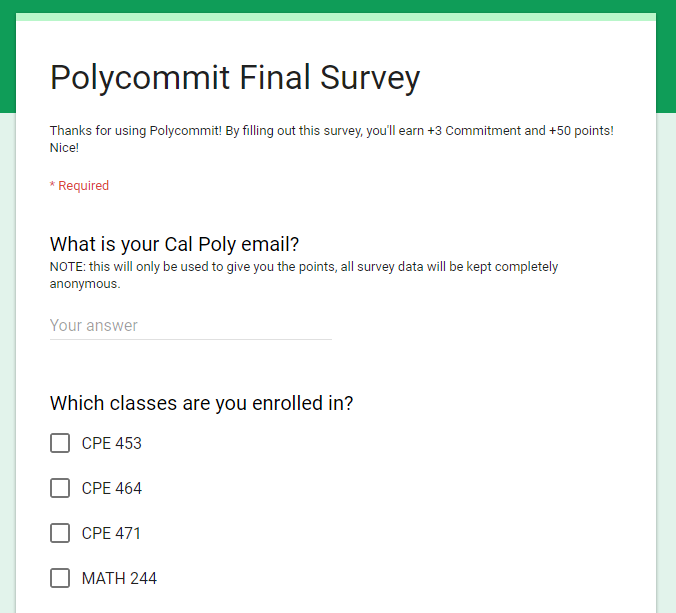
\includegraphics[width=1.0\linewidth]{figures/survey1}
	\label{fig:survey1}
\end{figure}

\begin{figure}[h!]
	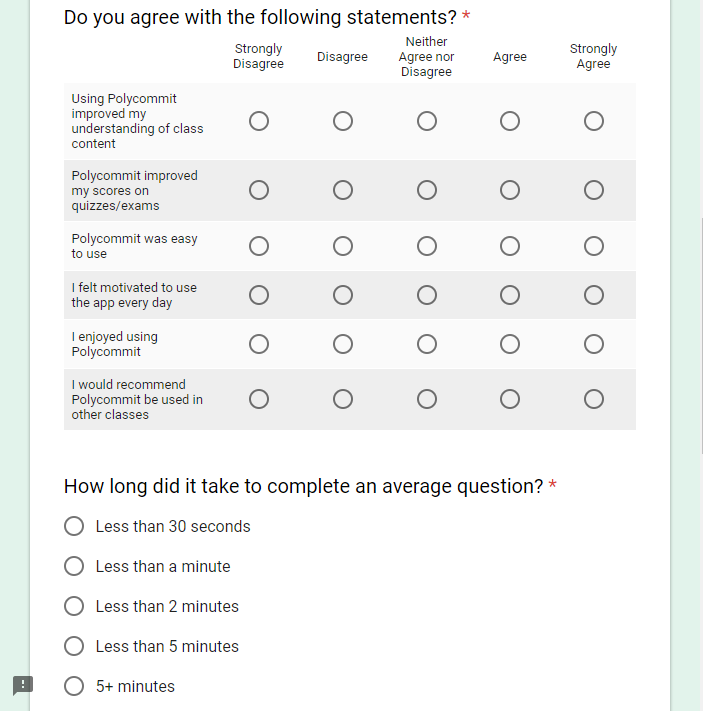
\includegraphics[width=1.0\linewidth]{figures/survey2}
	\label{fig:survey2}
\end{figure}

\begin{figure}[h!]
	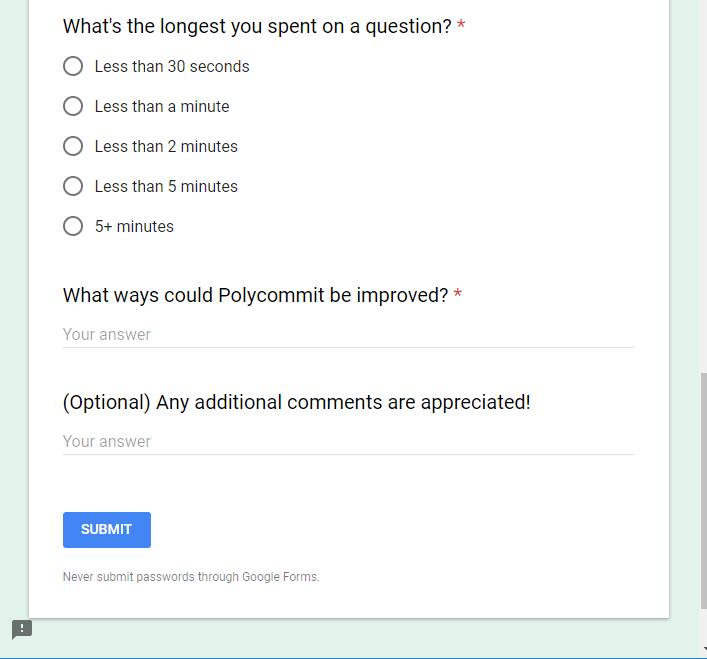
\includegraphics[width=1.0\linewidth]{figures/survey3}
	\label{fig:survey3}
\end{figure}
